\section{Top Quark Pair Background} \label{sec:background:ttbar}

The substantial contribution to the SR by boosted $t\bar{t}$ production shown
in \Cref{table:efficiencies_and_yields} makes its modeling a top
priority~\footnote{Pun!}.  Unfortunately, current MC generators are not able to
predict the $t\bar{t}$ cross section well in this boosted regime as seen in
\Cref{sec:background:mismodeling}.  This long-standing issue is likely due to
missing higher-order diagrams rather than due to suboptimal generator setup
\cite{ATL-PHYS-PUB-2018-009}.  To compensate for this mismodeling the
$t\bar{t}$ yield in the SR is corrected with a normalization scale factor.  The
scale factor, or $k$-factor, is derived by fitting the $t\bar{t}$ normalization
in the $t\bar{t}$ enriched control region ($\text{CR}_{t\bar{t}}$).  In the
final fit the SR $t\bar{t}$ MC sample is fit by a double-sided Crystal Ball
function \cite{Gaiser:1982yw} to smooth out statistical fluctuations, and then
its normalization is constrained with the derived flat $k$-factor using its
uncertainty.

\begin{figure}[!htbp]
\centering
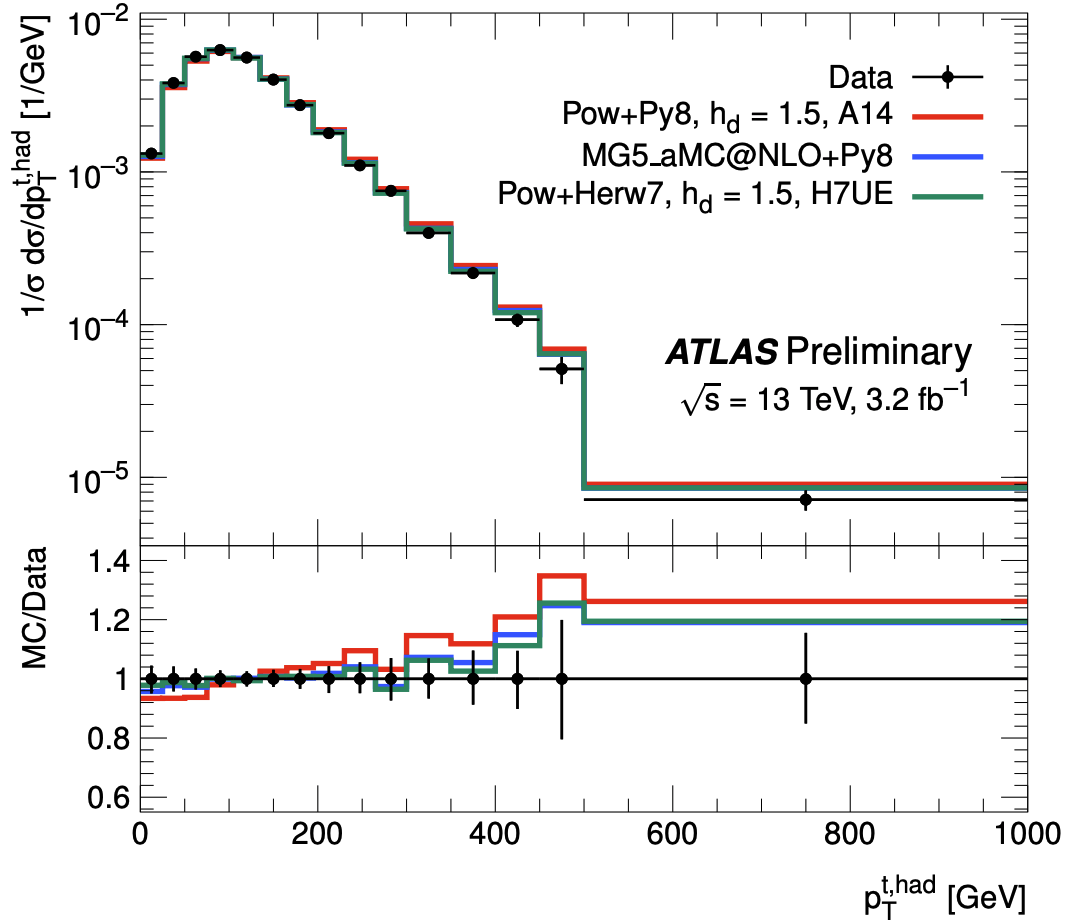
\includegraphics[width=0.6\linewidth]{figures/backgrounds/mismodeling}
\caption{Comparison in $\pT$ of the top quark for different generator setups
used to assess the NLO+PS matching as well as the parton shower and
hadronization uncertainty after optimization, compared to data at $\sqrt{s} =
13~\TeV$ \cite{ATL-PHYS-PUB-2018-009}.}
\label{sec:background:mismodeling}
\end{figure}

\subsection{Constructing the $\text{CR}_{t\bar{t}}$ Control Region}

The $t\bar{t}$-enriched control region uses the same $\pT$ selections as the
signal candidate large-$R$ jet in addition to the following criteria to select
$t\bar{t}$ events like the one shown in \Cref{sec:background:ttbar_depiction}.
Three regions are defined by requiring zero ($\text{CR}_{t\bar{t}0}$), one
($\text{CR}_{t\bar{t}}$) or two ($\text{CR}_{t\bar{t}2}$) tight quality
$b$-tags in the two leading VR track jets of the signal candidate. The
configuration with exactly one $b$-tag, $\text{CR}_{t\bar{t}}$, was chosen
to exploit the single $b$-quark that results from the dominant decay mode of
the top quark $t \rightarrow bW$.  This one $b$-tag region has contributions from
$t\bar{t}$, single-top, $Z$ and $H$ when one $b$-tag is lost, and multijet when
the $b$-tag is faked.  The other two regions are used to validate the
extrapolation of the $k$-factor into the $\text{CR}_{\text{QCD}}$ and SR.

\begin{figure}[!htbp]
  \centering
\subcaptionbox{\label{sec:backgrounds:ttbar_feynman}}{
\resizebox{0.48\linewidth}{!}{
\begin{tikzpicture}
  \begin{feynman}
    % initial state particles
    \vertex (i1) {\(q\)};
    \vertex [below=2cm of i1] (i2) {\(\bar{q}\)};

    % vertices
    \vertex [below right=1.cm and 1cm of i1] (a);
    \vertex [right=0.7cm of a] (b);

    % final state particles
    \vertex [above right=0.3cm and 0.5cm of b] (t1);
    \vertex [below right=0.3cm and 0.5cm of b] (t2);

    \vertex [above right=0.7cm and 0.7cm of t1] (W1);
    \vertex [blue, right=1.0cm of t1] (f1) {\(\bar{b}\)};

    \vertex [blue, right=1.0cm of t2] (f2) {\(b\)};
    \vertex [below right=0.7cm and 0.7cm of t2] (W2);

    \vertex [above right=0.1cm and .6cm of W1] (f3) {\(\bar{\nu}_{\mu}\)};
    \vertex [below right=0.1cm and .6cm of W1] (f4) {\(\mu^{-}\)};
    \vertex [above right=0.1cm and .6cm of W2] (f5) {\(\bar{q}\)};
    \vertex [below right=0.1cm and .6cm of W2] (f6) {\(q\)};

    \diagram* {
      (i1) -- [fermion] (a) 
        -- [fermion] (i2),

      (a) -- [gluon, edge label'=\(g\)] (b),

      (t1) -- [orange, fermion, edge label'=\(\bar{t}\)] (b)
        -- [orange, fermion, edge label'=\(t\)] (t2),

      (f1) -- [blue, fermion] (t1)
        -- [red, boson, edge label=\(W^{-}\)] (W1),
      (f2) -- [blue, anti fermion] (t2)
        -- [red, boson, edge label'=\(W^{+}\)] (W2),

      (f3) -- [fermion] (W1)
        -- [fermion] (f4),
      (f5) -- [fermion] (W2)
        -- [fermion] (f6),
    };

      
  \end{feynman}
\end{tikzpicture}
}} \hfill
\subcaptionbox{\label{sec:backgrounds:ttbar_cartoon}}{
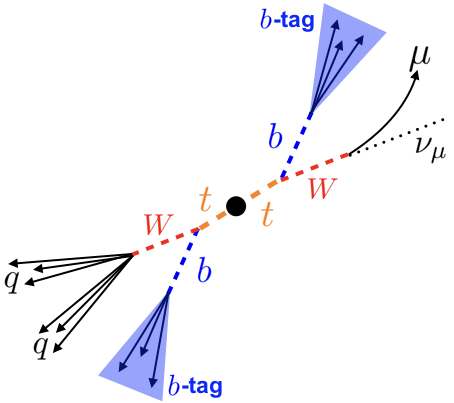
\includegraphics[width=0.48\linewidth]{figures/backgrounds/ttbar_cartoon}
}

\caption{(a) Feynman diagram of semi-leptonic $t\bar{t}$ decay. (b) Cartoon depicting semi-leptonic $t\bar{t}$ decay to $b$-quarks in center of mass frame.}
\label{sec:background:ttbar_depiction}

\end{figure}

To reduce multijet contamination in the sample the second top quark in the
opposite hemisphere of the signal candidate is required to decay leptonically
in the muon channel. \Cref{sec:backgrounds:phi_study} compares the $\Delta\phi$
between the leading muon in the event and the signal candidate jet for the
multijet and $t\bar{t}$ MC samples. This distribution shows the expected
back-to-back topology of the $t\bar{t}$ system depicted in
\Cref{sec:backgrounds:ttbar_cartoon} versus the multijet sample where the muons
come from the signal candidate due to hadron decays in flight. Thus, a cut of
$\Delta\phi(\text{muon} - \text{signal}) > \frac{2\pi}{3}$ was
chosen\footnote{Note that while the dotted magenta line in
\Cref{sec:backgrounds:phi_study} technically indicates an optimal
$\Delta\phi(\text{muon} - \text{signal})$ cut of 1.09956, practically a cut of
$\frac{2\pi}{3}$ was chosen to reject as much multijet background as possible.}
to reduce the QCD contribution by several orders of magnitude while only
reducing the $t\bar{t}$ contribution by roughly a factor of five.

The QCD contribution is further suppressed by requiring the muon $\pT >40~\GeV$.
\Cref{sec:backgrounds:pt_study} compares the $\pT$ spectra for $t\bar{t}$ and
QCD before the $\Delta\phi$ cut selection. The larger mass of the $W$
boson leads to higher $\pT$ muons than the softer x muons from heavy flavor jets.

\begin{figure}[!htbp]
\centering
\subcaptionbox{$\Delta \phi(\text{leading muon}-\text{signal})$ study \label{sec:backgrounds:phi_study}}{
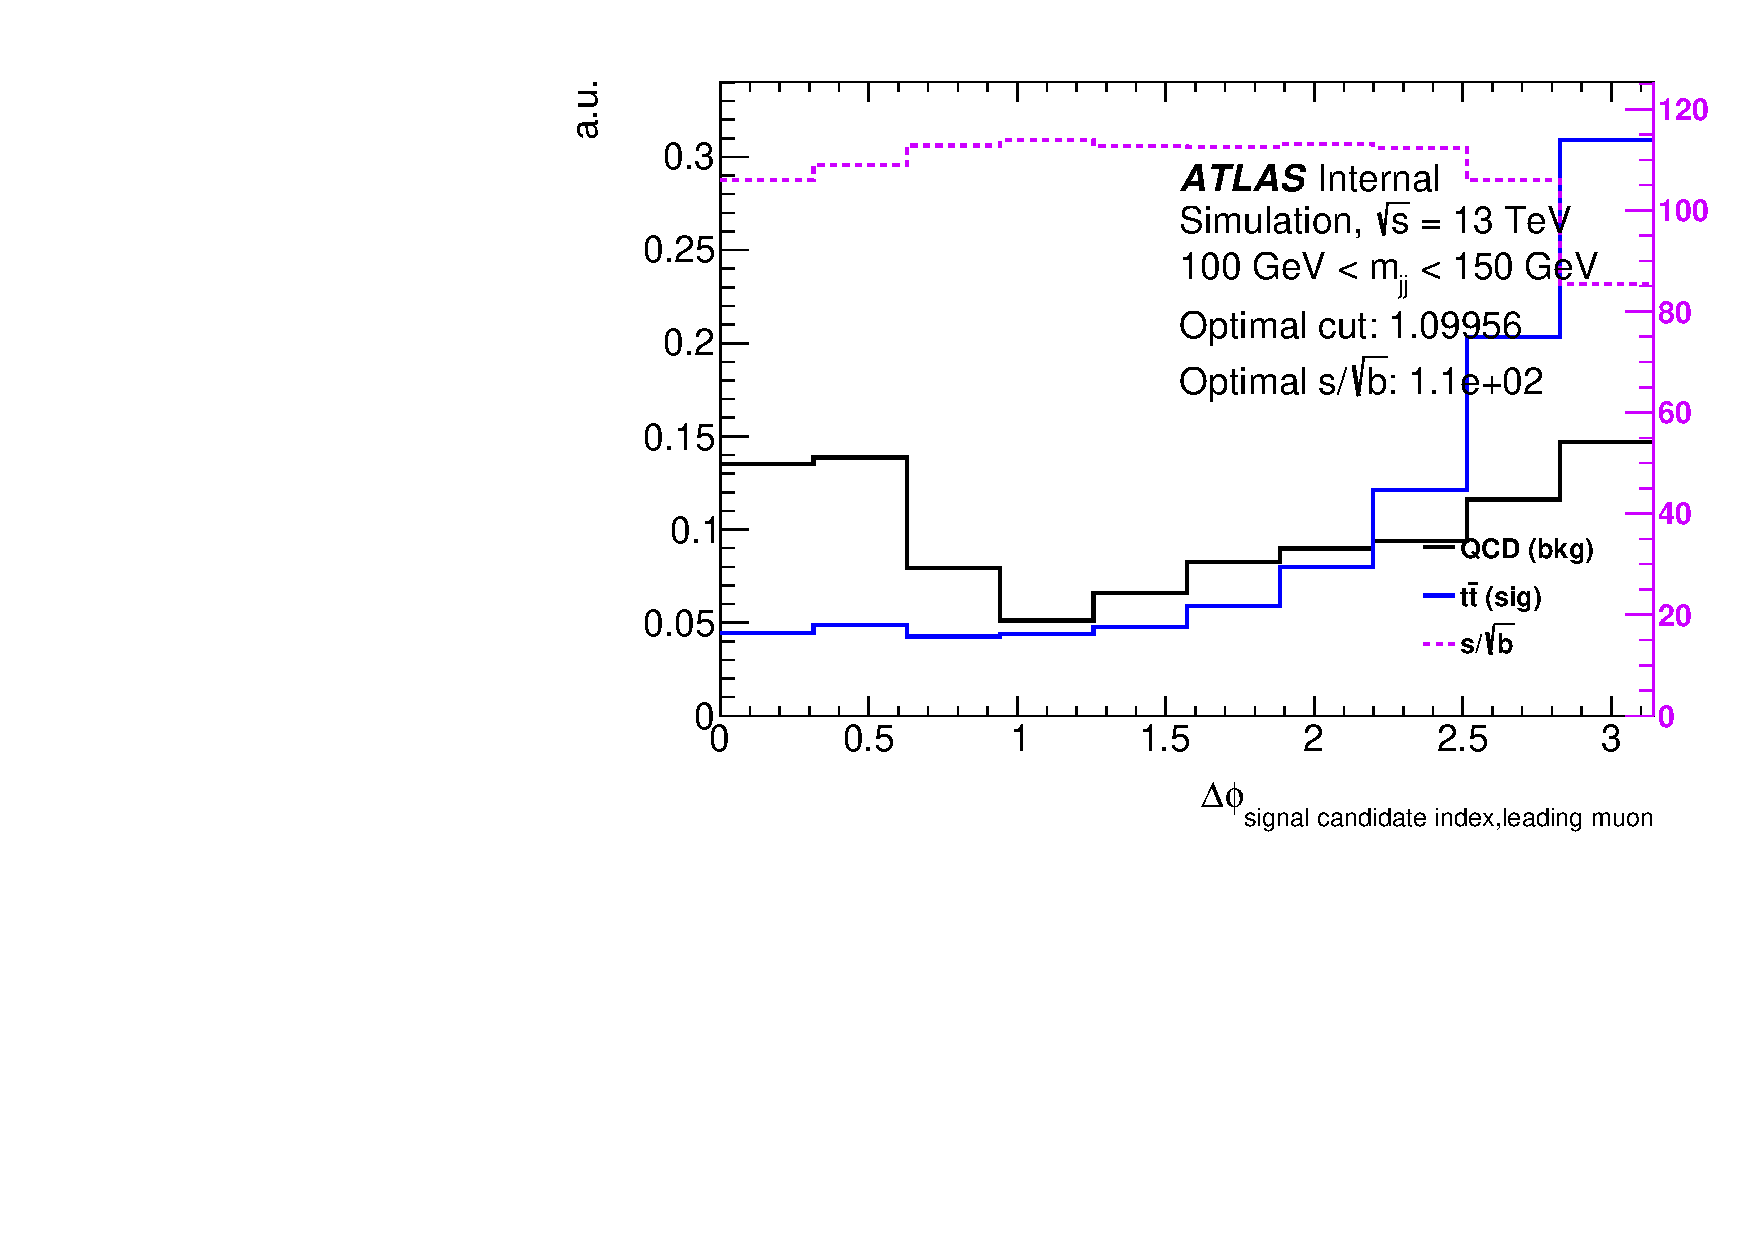
\includegraphics[width=0.48\linewidth]{figures/backgrounds/phi_study}
}\hfill
\subcaptionbox{Leading muon $\pT$ study \label{sec:backgrounds:pt_study}}{
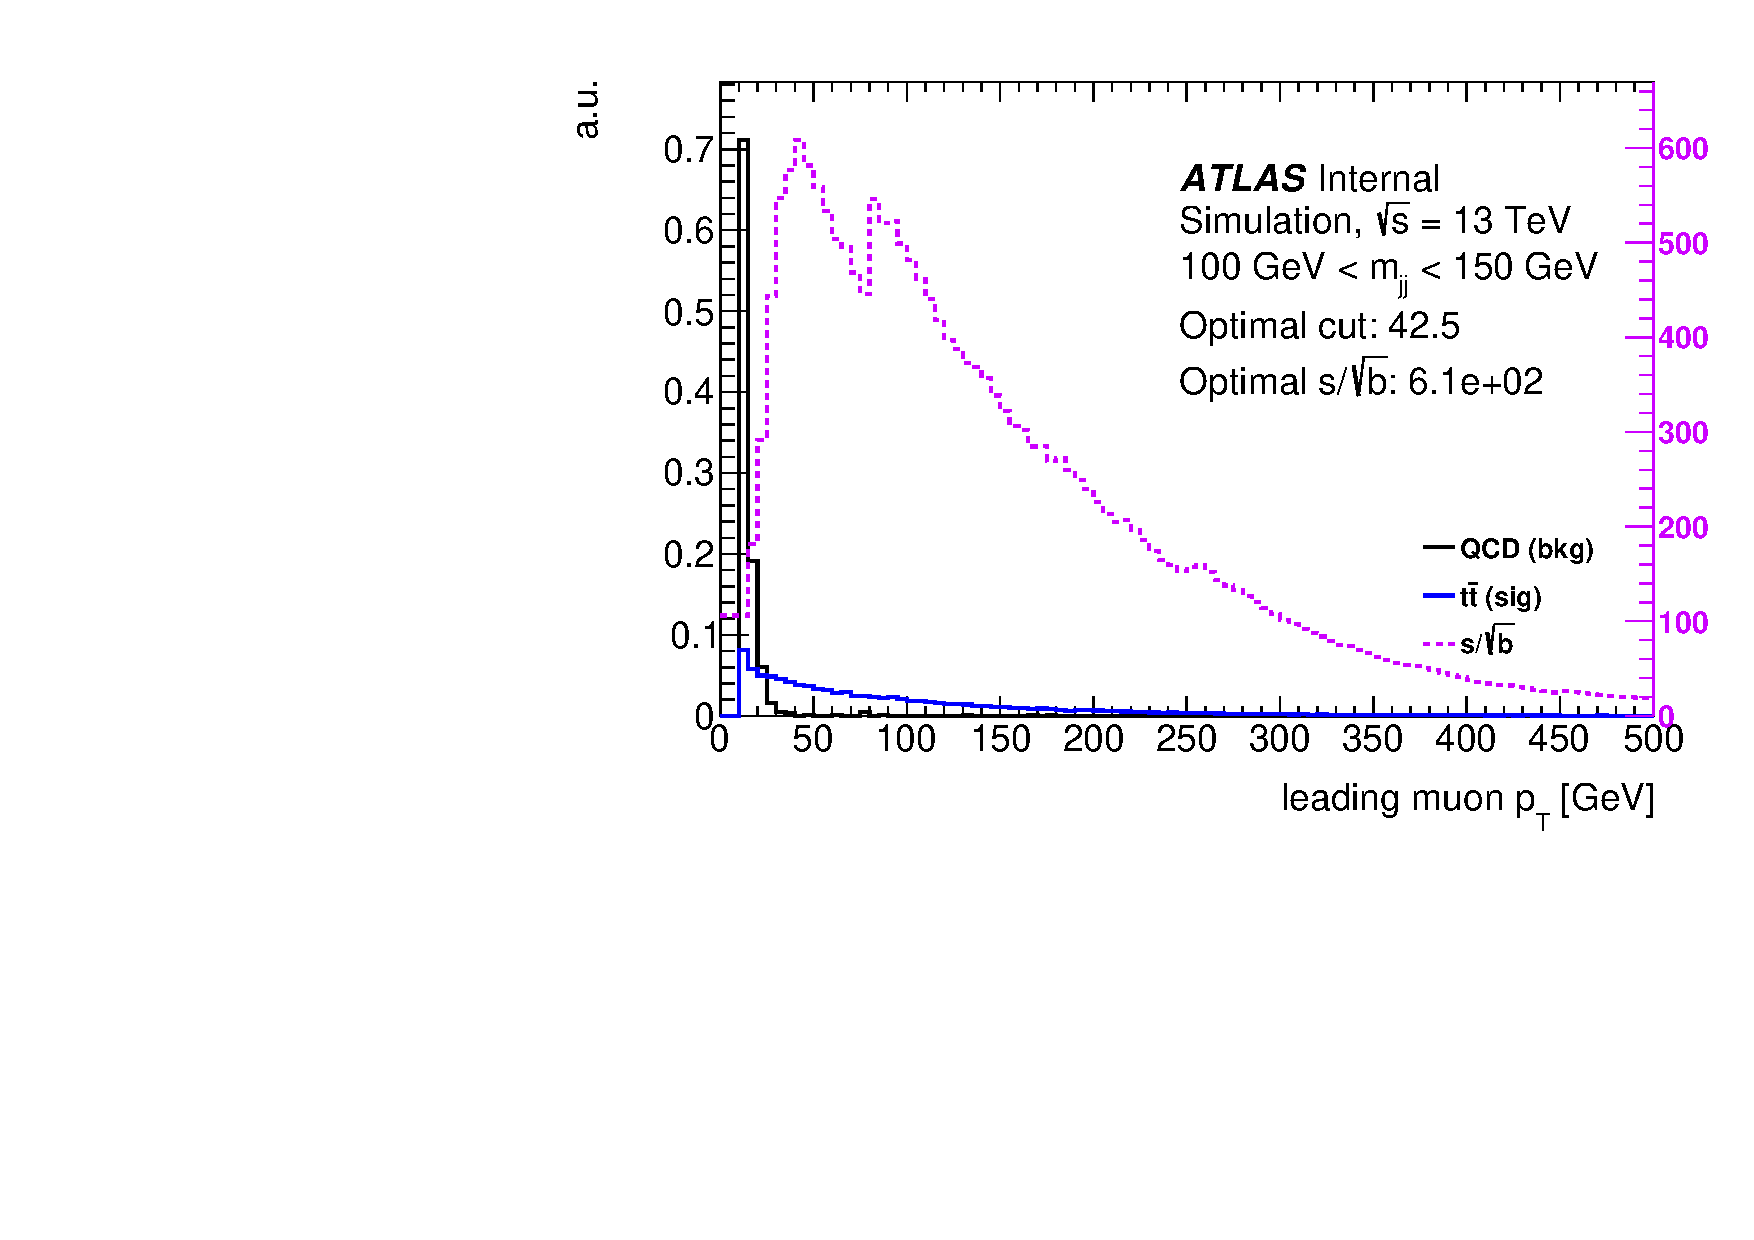
\includegraphics[width=0.48\linewidth]{figures/backgrounds/pt_study}
}
\caption{Comparison of the two variables, $\Delta \phi(\text{leading muon}-\text{signal})$ (a) and muon $\pT$ (b), between \textsc{Pythia}8 multijet and \textsc{Powheg} \ttbar simulated events used to create the \ttbar control region. The selection requires exactly one $b$-tagged track jet in the signal candidate \largeR jet. The magenta line shows the expected $s/\sqrt{b}$ significance with $80.5~\ifb$ \cite{Krizka:2310645}.}
\label{sec:background:qcd_rejection_studies}
\end{figure}

Finally, at least one tight $b$-tagged track-jet is required to be within
$\Delta R < 1.5$ of the chosen muon.  This requirement exploits the collimation
of the decay products of the boosted top quark $t \rightarrow
b\mu\nu_{\mu}$.  This reduces the contamination from $V(ll)$+jets
and $VV$ events. The above $\text{CR}_{t\bar{t}}$ selections are summarized visually in \Cref{sec:background:ttbar_selection_diagram}.

\begin{figure}[!htbp]
\centering
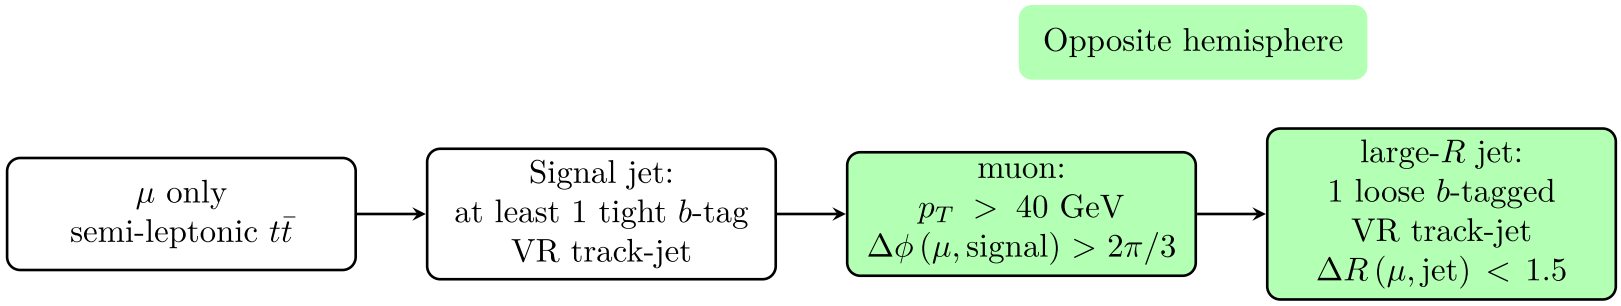
\includegraphics[width=1.0\linewidth]{figures/backgrounds/ttbar_selection}
\caption{Diagram of the $\text{CR}_{t\bar{t}}$ selection criteria \cite {Feickert:2690521}.}
\label{sec:background:ttbar_selection_diagram}
\end{figure}

\subsection{$k$-factor Estimation}

Finally the $t\bar{t}$ MC template is fit to the data in the
$\text{CR}_{t\bar{t}}$ over the mass range $100~\GeV$ to $200~\GeV$.  Single
top ($Wt$) and $W \rightarrow l\nu$ templates were included in the fit with
their normalizations kept constant. The full statistical and systematic
uncertainty is determined by running the Bayesian Analysis Toolkit (BAT)
\cite{Beaujean:2011zz}, discussed in \Cref{chap:fit}, with the large-$R$ jet
energy scale (JES), jet mass resolution (JMR), luminosity, $t\bar{t}$
modeling and flavor tagging systematic uncertainties discussed in
\Cref{chap:systematics}.

The pre- and post-fit distributions for the $\text{CR}_{t\bar{t}}$ are shown in
\Cref{sec:background:ttbar_fit} with the pull distributions shown in
\Cref{sec:background:ttbar_pulls}.  The JES and JMR systematics are constrained
by information about the peak in $t\bar{t}$ which was not available in the
dataset used to derive the recommendations\footnote{Note that the
$\text{CR}_{t\bar{t}}$ and final fit are not simultaneous so these JES and JMR
constraints do not affect the final fit.}. A systematic uncertainty dominated
$k$-factor of $0.84 \pm 0.11$ is found for $\text{CR}_{t\bar{t}}$, showing that
the MC overestimates the $t\bar{t}$ yield as expected (see
\Cref{sec:background:mismodeling}). This value is used to constrain the
$t\bar{t}$ contribution in the final fit to the SR. The results for all three
$t\bar{t}$ control regions are given in \Cref{table:ttbar_kfactors}.  All three
regions are consistent with each other and the results presented in reference
\cite{ATLAS:2016jct}.

\begin{table}
  \centering
  \caption{The \ttbar scale factors and their uncertainties from the three \ttbar
control regions. The value for $\text{CR}_{t\bar{t}}$ is used in the Signal Region. NOTE:
$\text{CR}_{t\bar{t}2}$ fit failed due to low statistics but is almostly completely dominated
by ttbar in this region.  The value here is the simple ratio of number of events in ttbar
vs. data, and the uncertainty is the $t\bar{t}$ statistical uncertainty.}
  \begin{tabular}{@{}lrr@{}}
    \toprule
    Region & scale factor & uncertainty \\
    \midrule
    $\text{CR}_{t\bar{t}0}$ & $0.87$ & $0.12$ \\
    $\text{CR}_{t\bar{t}}$  & $0.84$ & $0.11$ \\
    $\text{CR}_{t\bar{t}2}$ & $0.96$ & $0.21$ \\
    \bottomrule
  \end{tabular}
  \label{table:ttbar_kfactors}
\end{table}

\begin{figure}[!htbp]
\centering
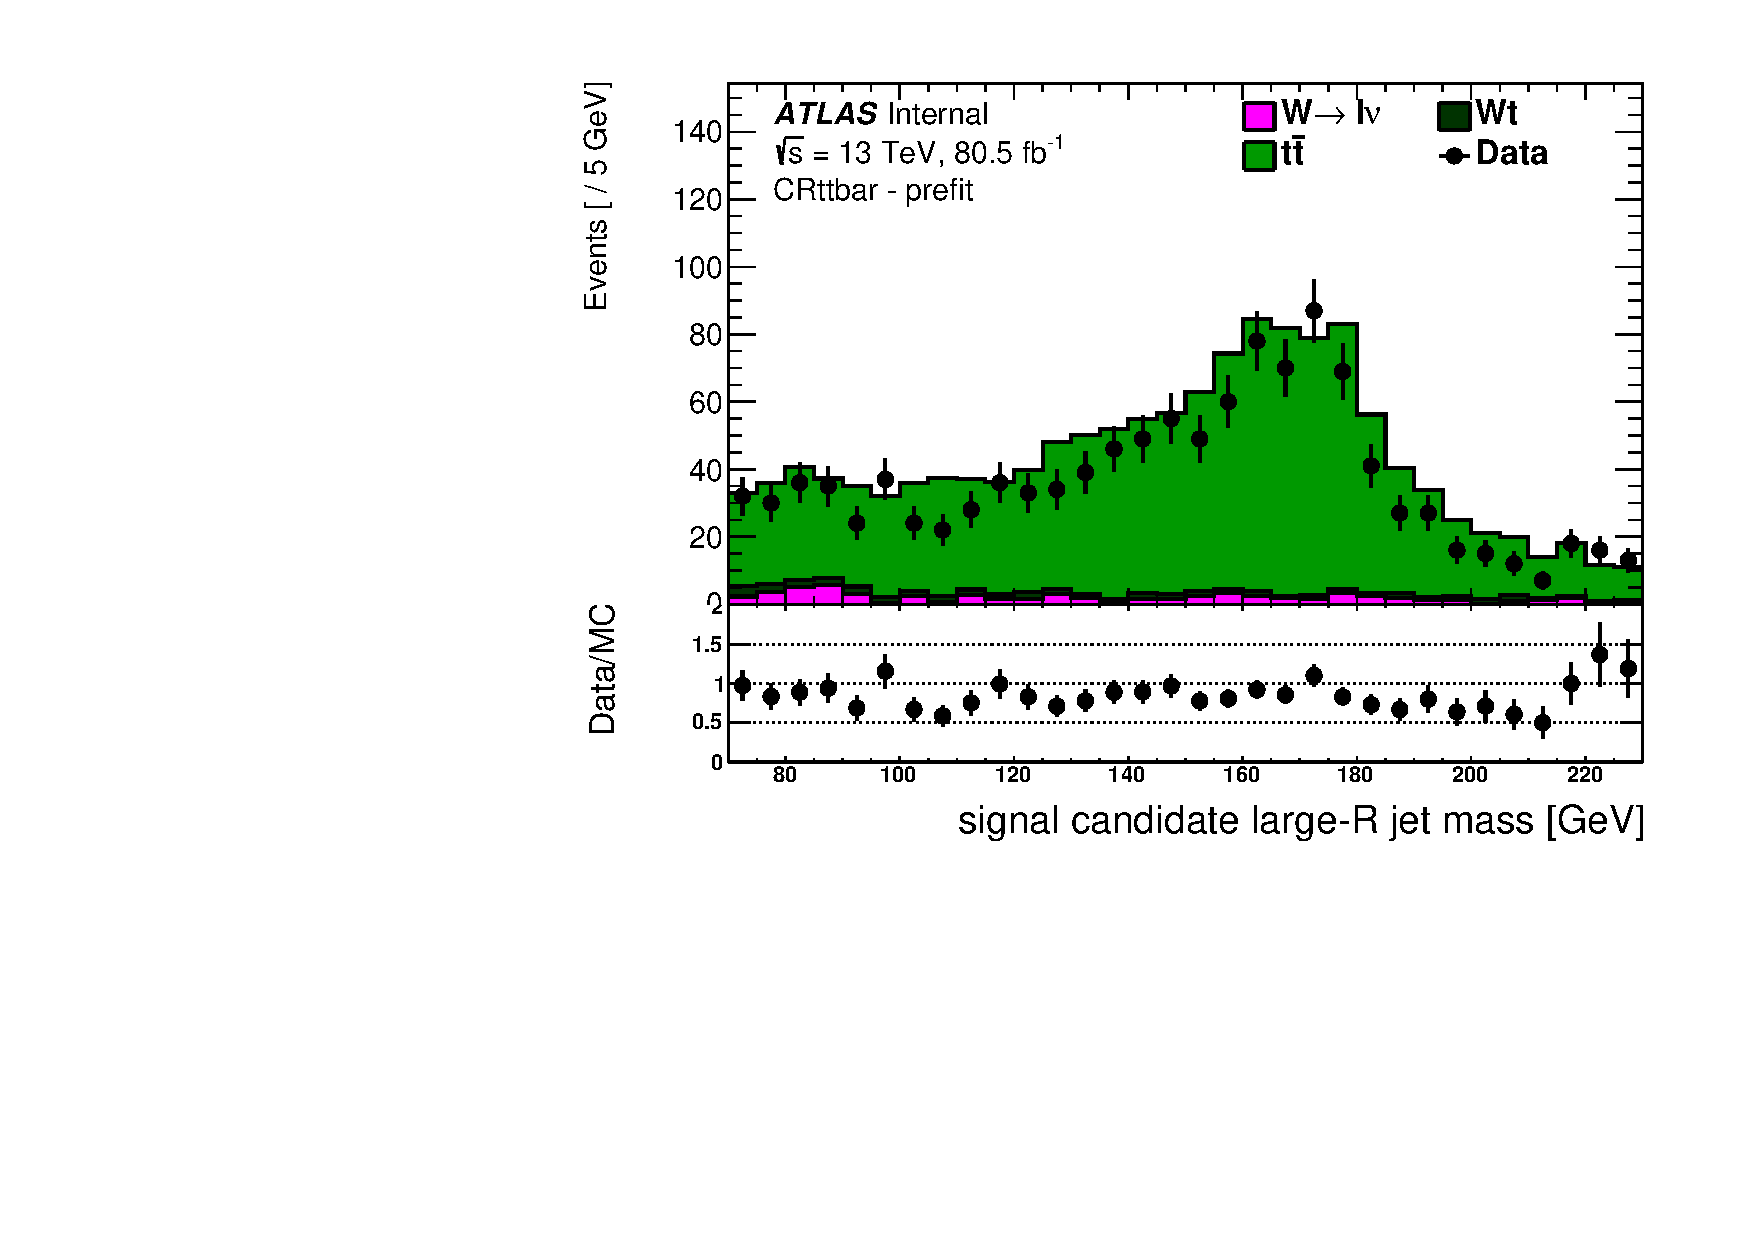
\includegraphics[width=0.49\linewidth]{figures/backgrounds/ttbar_prefit} \hfill
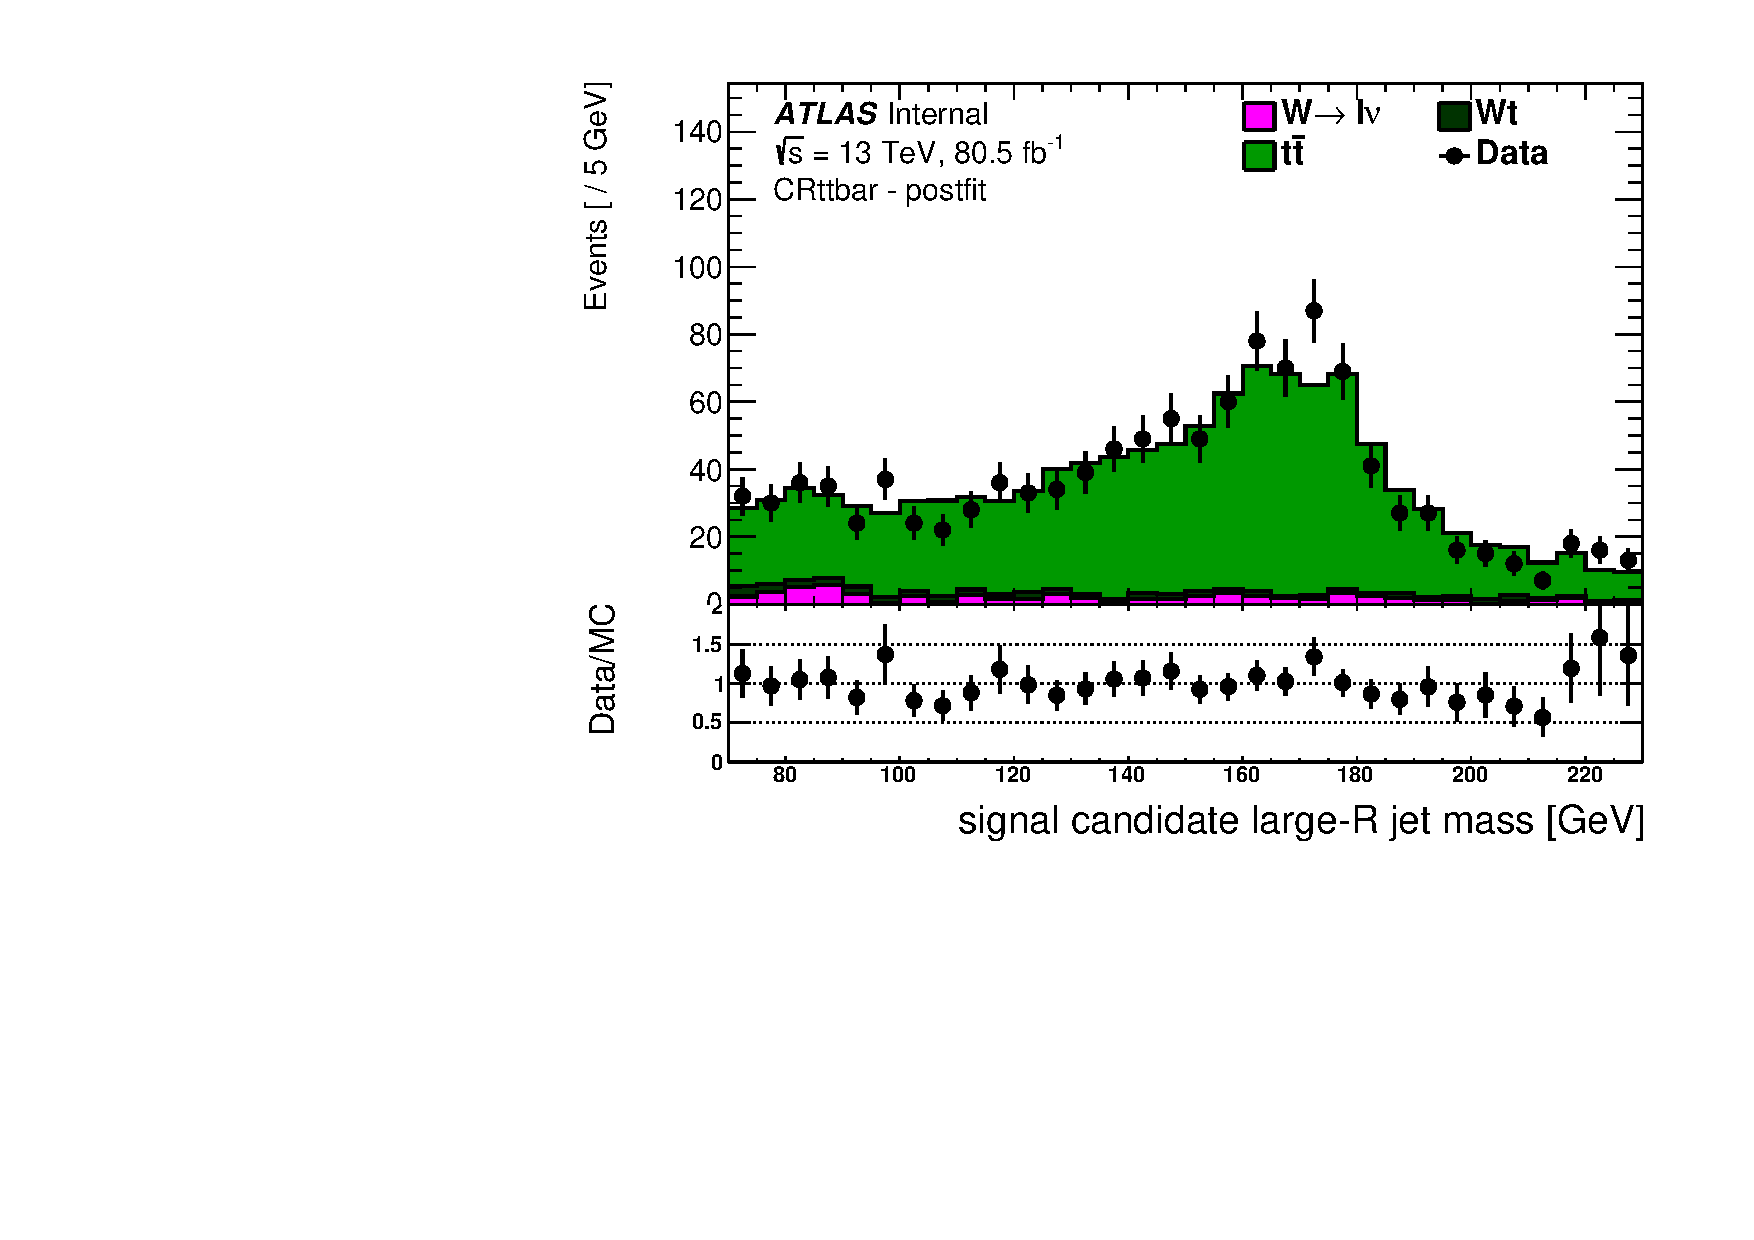
\includegraphics[width=0.49\linewidth]{figures/backgrounds/ttbar_postfit}
\caption{The pre-fit (left) and post-fit (right) data vs MC comparison for fitting the $\text{CR}_{t\bar{t}}$ region.}
\label{sec:background:ttbar_fit}
\end{figure}

\begin{figure}[!htbp]
\centering
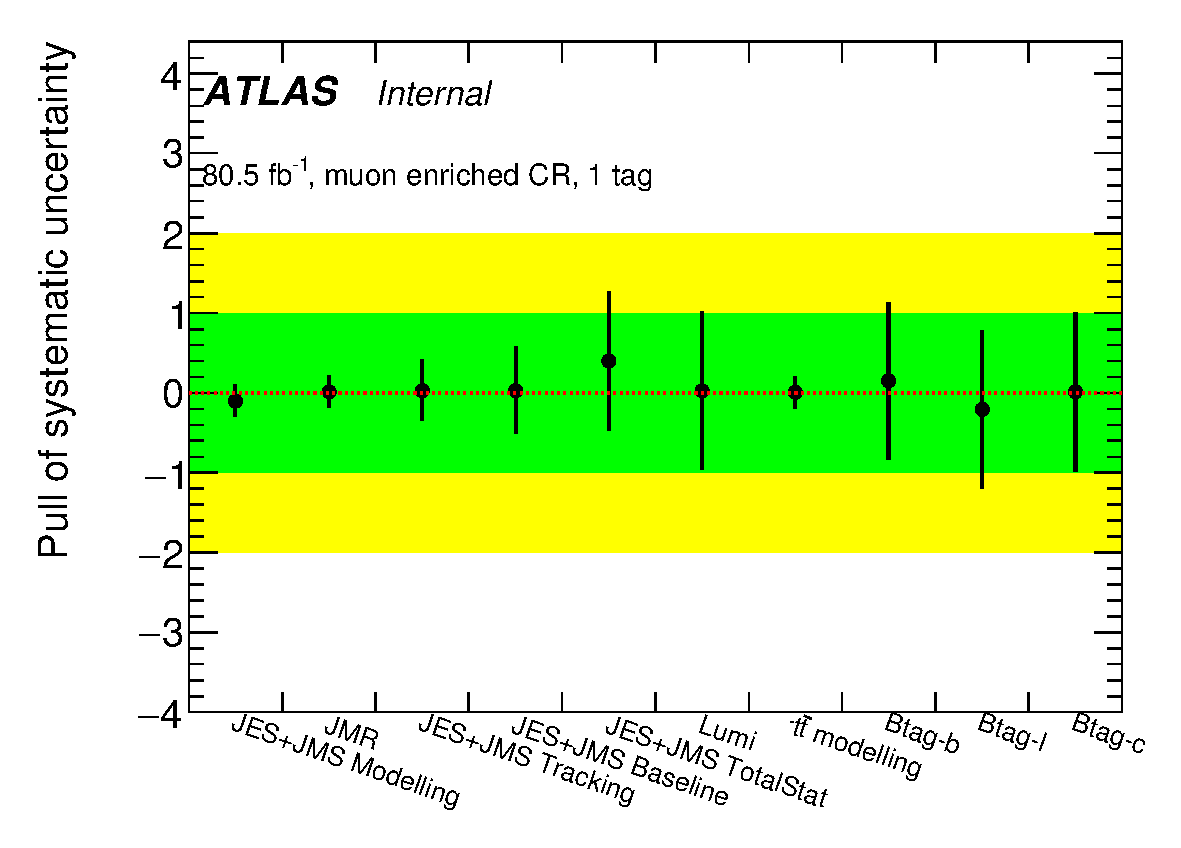
\includegraphics[width=0.7\linewidth]{figures/backgrounds/ttbar_pulls}
\caption{The pull distributions for the different nuisance parameters used in the $\text{CR}_{t\bar{t}}$ fit. Parameters with a error less than 1 indicate that the prior uncertainty has been constrained by the fit.}
\label{sec:background:ttbar_pulls}
\end{figure}
